\chapter{Software Development}
\label{chap:software-development}

% \section{Software Development Methodology}
% \label{section:software-development-methodology}
% <TIP: Describe your software development methodology in this section. />

% \section{Technology Stack}
% \label{section:technology-stack}
% <TIP: Describe your technology stack here. See the following example from ThaiProgrammer.org />
% \begin{figure}[h]
%     \centering
%     
\includegraphics[width=0.5\textwidth]{examples/tech-stack.png}
%     \caption{Example technology stack}
% \end{figure}

% \section{Coding Standards}
% \label{section:coding-standards}
% <TIP: Describe your coding standard for this project here. />

\section{Schedule}
\label{section:schedule}
\begin{figure}[ht]
    \centering
    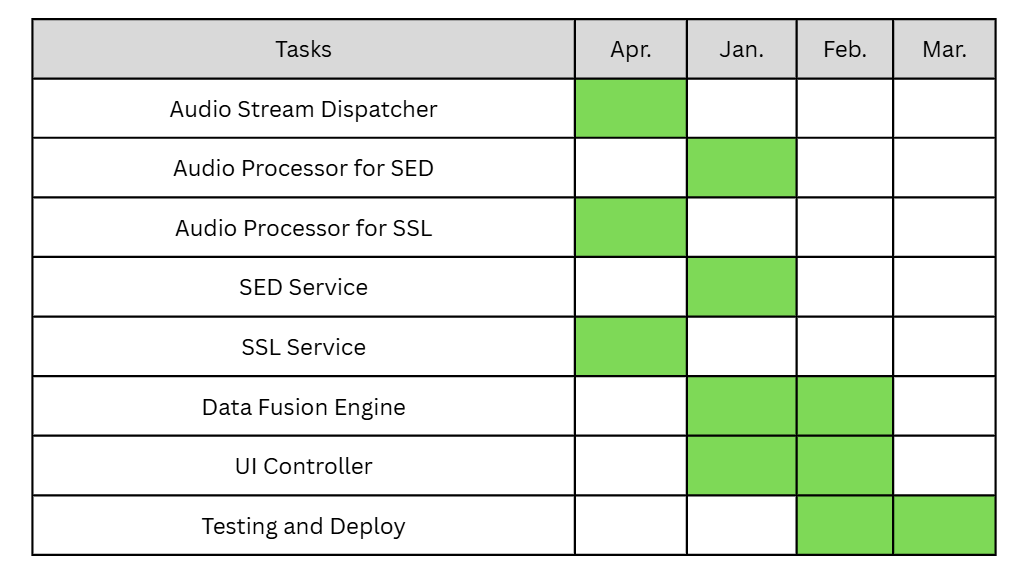
\includegraphics[width=1\textwidth, height=8cm, keepaspectratio]{assets/timeline/timeline.png}
    \caption{Project Schedule.}
\end{figure}

The development of Sonar Retina follows a modular, priority-based timeline to ensure high precision and low latency in critical AI components.

\textbf{Phase 1: SSL and Initial Mobile Interface Development (April 2026):}  
The first phase focuses on the development of the Sound Source Localization (SSL) infrastructure. 
This includes implementing the \textit{Audio Processor} for phase-difference analysis and the core \textit{SSL Service}. 
In parallel, the initial version of the mobile interface will be developed to support basic visualization and interaction with localization outputs.

\textbf{Phase 2: SED, Data Fusion, and Mobile Expansion (January 2027):}  
The second phase focuses on the Sound Event Detection (SED) components. 
This includes implementing the \textit{Audio Stream Dispatcher}, the \textit{Audio Processor} optimized for spectrogram extraction, and the core \textit{SED Service}. 
At the same time, development of the \textit{Data Fusion Engine} will begin to synchronize semantic and spatial information from both AI services. 
Further improvements and feature expansion of the mobile interface will also be carried out during this phase.

\textbf{Phase 3: Final Integration and Deployment (February and March 2027):}  
The final phase focuses on refining the \textit{UI Controller} and completing the \textit{Data Fusion Engine} to ensure seamless visualization and synchronization of results within the Radar UI. 
The project concludes in March 2027 with full system integration, deployment, and comprehensive validation.
% \section{Progress Tracking Report}
% \label{section:progress-tracking-report}
% <TIP: Show that you have been working on this project overtime.
% It can be in the form of a burndown chart or a contribution graph from GitHub./>